\textbf{Zmodyfikowany model podstawowy uczony na grafach sześciowierzchołkowych}

% -- TO DO -- % Opis modyfikacji

% -- TO DO -- % Dokładność

% -- TO DO -- % Strata

\begin{figure}[ht]
	\centering
	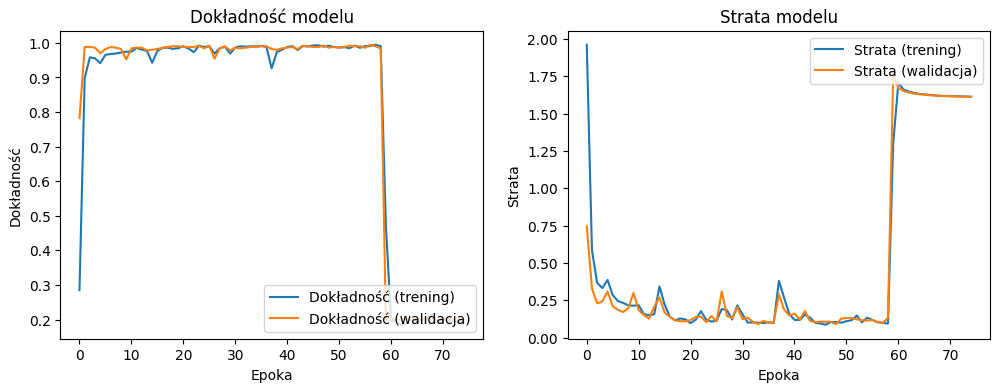
\includegraphics[height=5.5cm]{resources/tests/images/v4/base6_1_img.png}
	\caption{Wyniki testów dla zmodyfikowanego modelu podstawowego, liczba wierzchołków = 6}
	\label{Fig:tests-base-5a}
\end{figure}
\FloatBarrier

% \begin{figure}[ht]
% 	\centering
% 	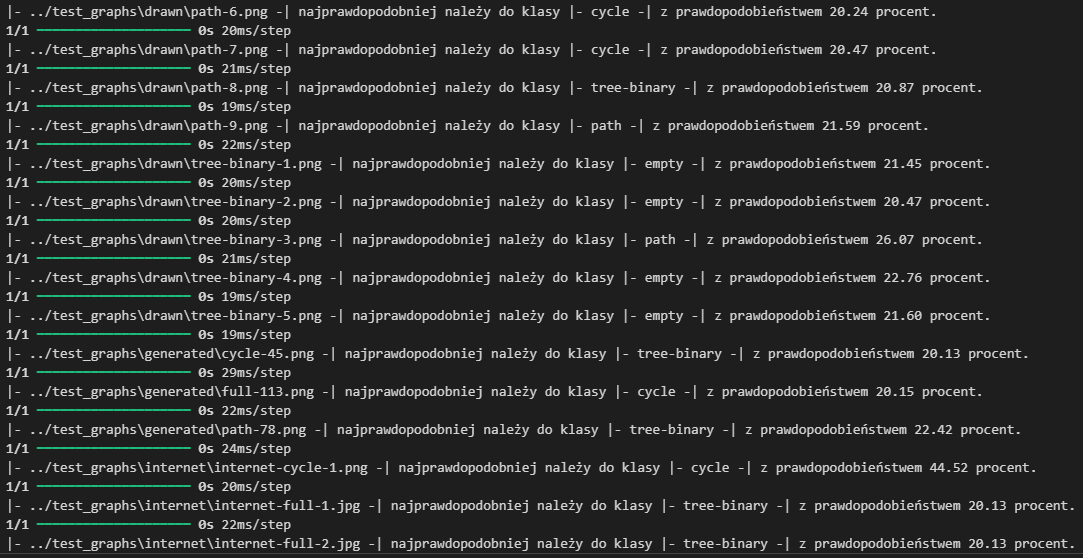
\includegraphics[width=14cm]{resources/tests/images/v4/base6_1_txt.png}
% 	\caption{Klasyfikacja obrazów zewnętrznych dla zmodyfikowanego modelu podstawowego, liczba wierzchołków = 6}
% 	\label{Fig:tests-base-5b}
% \end{figure}
% \FloatBarrier

% \begin{figure}[ht]
% 	\centering
% 	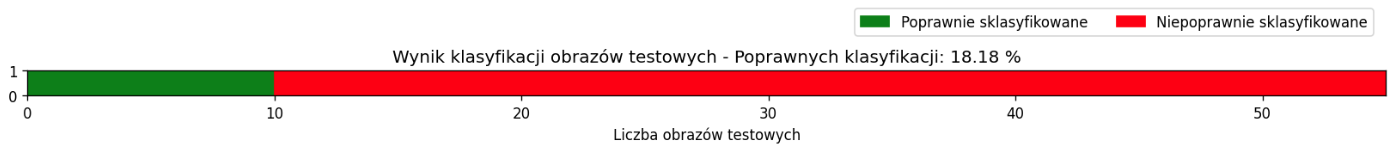
\includegraphics[width=14cm]{resources/tests/images/v4/base6_1_bar.png}
% 	\caption{Wizualizacja klasyfikacji obrazów zewnętrznych dla zmodyfikowanego modelu podstawowego, liczba wierzchołków = 6}
% 	\label{Fig:tests-base-5c}
% \end{figure}
% \FloatBarrier

\textbf{Zmodyfikowany poprawiony model podstawowy uczony na grafach sześciowierzchołkowych}

% -- TO DO -- % Opis modyfikacji

% -- TO DO -- % Dokładność

% -- TO DO -- % Strata

\begin{figure}[ht]
	\centering
	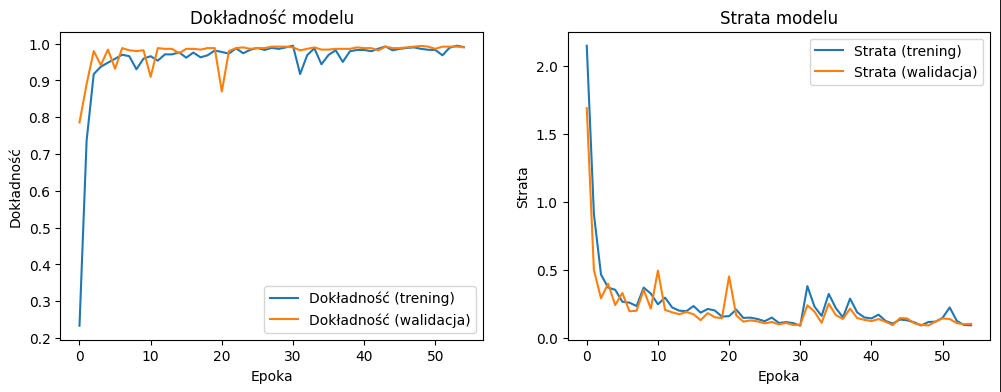
\includegraphics[height=5.5cm]{resources/tests/images/v4/base6_1_1_img.png}
	\caption{Wyniki testów dla poprawionego zmodyfikowanego modelu podstawowego, liczba wierzchołków = 6}
	\label{Fig:tests-base-6a}
\end{figure}
\FloatBarrier

% -- TO DO -- % Opis ogólny

\begin{figure}[ht]
	\centering
	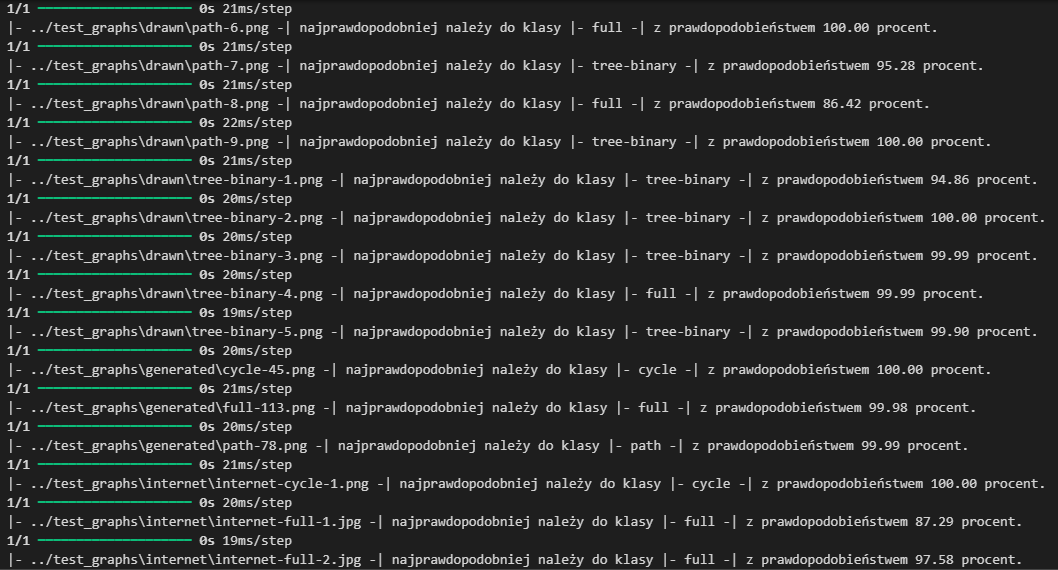
\includegraphics[width=14cm]{resources/tests/images/v4/base6_1_1_txt.png}
	\caption{Klasyfikacja obrazów zewnętrznych dla poprawionego zmodyfikowanego modelu podstawowego, liczba wierzchołków = 6}
	\label{Fig:tests-base-6b}
\end{figure}
\FloatBarrier

\begin{figure}[ht]
	\centering
	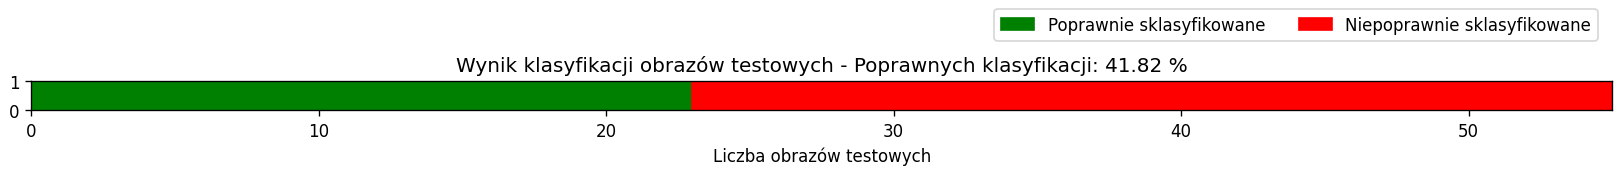
\includegraphics[width=14cm]{resources/tests/images/v4/base6_1_1_bar.png}
	\caption{Wizualizacja klasyfikacji obrazów zewnętrznych dla poprawionego zmodyfikowanego modelu podstawowego, liczba wierzchołków = 6}
	\label{Fig:tests-base-6c}
\end{figure}
\FloatBarrier

% -- TO DO -- % Opis klasyfikacji